% !Mode:: "TeX:UTF-8"
% !TEX program  = xelatex

% \documentclass{cumcmthesis}
\documentclass[withoutpreface,bwprint]{cumcmthesis} %去掉封面与编号页,电子版提交的时候使用。

\usepackage{graphicx} %use graph format
\usepackage{epstopdf}
\usepackage[framemethod=TikZ]{mdframed}
\usepackage{url}   % 网页链接
\usepackage{subcaption} % 子标题
\title{全国大学生数学建模竞赛编写的 \LaTeX{} 模板}
\tihao{B}
\baominghao{12345678}
\schoolname{同济大学}
\membera{ }
\memberb{ }
\memberc{ }
\supervisor{ }
\yearinput{2020}
\monthinput{08}
\dayinput{22}

\begin{document}

 \maketitle
 \begin{abstract}
(抄的简介)
    当外部环境变化甚至不确定的情况下时,如何利用有限的资源在有限的时间内、有额外约束的情况下最大化收益,
    一直是管理科学领域研究的重要课题。
    本文对B题中的问题进行讨论,该问题是一个在沙漠中旅行的挖矿的游戏,需要在有限的时间内、确定或不确定的
    环境下、资源受限的情况下,作出合理的决策,从而最大化游戏的收益同时不保证失败。
    同时可能存在多个玩家共同决策的情况,各自的决策会相互影响。
    
    该问题需要综合动态规划、最短路径、不确定情况下最优决策和静态/动态博弈的思路建模解决。
    我们将在考虑用户可能会产生决策的关键结点的基础上,通过最短路径等思路简化网络后,建立动态规划的决策过
    程、不确定状态下的阶段性决策路径、以及动态博弈的关系,逐步解决该背景下的问题。

\keywords{最短路径\quad  动态规划\quad   动态决策\quad  博弈论}
\end{abstract}


\section{概述}
\subsection{问题背景}
\label{subsec:simulate}

当外部环境变化甚至不确定的情况下时,如何利用有限的资源在有限的时间内、有额外约束的情况下最大化收益,
一直是管理科学领域研究的重要课题。
本文对B题中的问题进行讨论,该问题是一个在沙漠中旅行的挖矿的游戏,需要在有限的时间内、确定或不确定的
环境下、资源受限的情况下,作出合理的决策,从而最大化游戏的收益同时不保证失败。
同时可能存在多个玩家共同决策的情况,各自的决策会相互影响。

该问题需要综合动态规划、最短路径、不确定情况下最优决策和静态/动态博弈的思路建模解决。
我们将在考虑用户可能会产生决策的关键结点的基础上,通过最短路径等思路简化网络后,建立动态规划的决策过
程、不确定状态下的阶段性决策路径、以及动态博弈的关系,逐步解决该背景下的问题。

\subsection{目标任务}

问题1:如何在天气已知的情况下,规划出最合适的路径,从而实现利润最大化。
我们建立了正向的动态规划模型,对用户的决策状态进行规划求解,目标函数是用户的利润,约束条件是必须在规
定的时间内到达目的地,且必须保证食物和水有剩余。
将该问题问题输入后,通过规划求解即可获得最优的用户策略。

问题2:如何在环境不确定的状态下作出最优决策,使得利润最大化。
我们建立了完整的决策路径,包括初始阶段、挖矿阶段、前往终点等多个决策阶段,计算了不同情况下的成本与利
润后,得出了不同决策阶段下、不同的环境下玩家应该作出的决策,使得在只知道当天天气的情况下,玩家能够获
得的收益最大化。

问题3:如何在多人参加且决策会互相影响的情况下,预先作出策略或根据环境作出最优策略。
我们建立了静态和动态的博弈模型,基于环境和用户决策的分析,计算了给定天气情况下,如何进行预先决策,使
得博弈获得收益最高;同时对用户的倾向进行分类,分析了在不同的选择倾向情况下,博弈的一般最佳策略。


\section{符号说明与模型基础}
\label{sec:simulate}

\subsection{模型简化}
\label{subsec:shortest}

在规划问题中,因为沙漠中大部分结点是等价的,除了“起点”、“终点”、“矿山”和“村庄”,以及部分用户可能会作出不同决策的
关键结点,其他结点可以进行简化。

为此,我们采用Dijkstra算法与匹配算法对模型进行简化。
首先将网络模型简化为点和邻接矩阵后,通过Dijkstra输出点与点之间的最短路径,同时通过匹配算法根据实际情况计算路径中
的重叠位置,并选择部分作为关键结点,比如第四关中,用户可以到达13号结点再决定前往矿山还是村庄,13号是关键结点。
具体算法参考附录A。

\begin{figure}[!h]
    \centering
    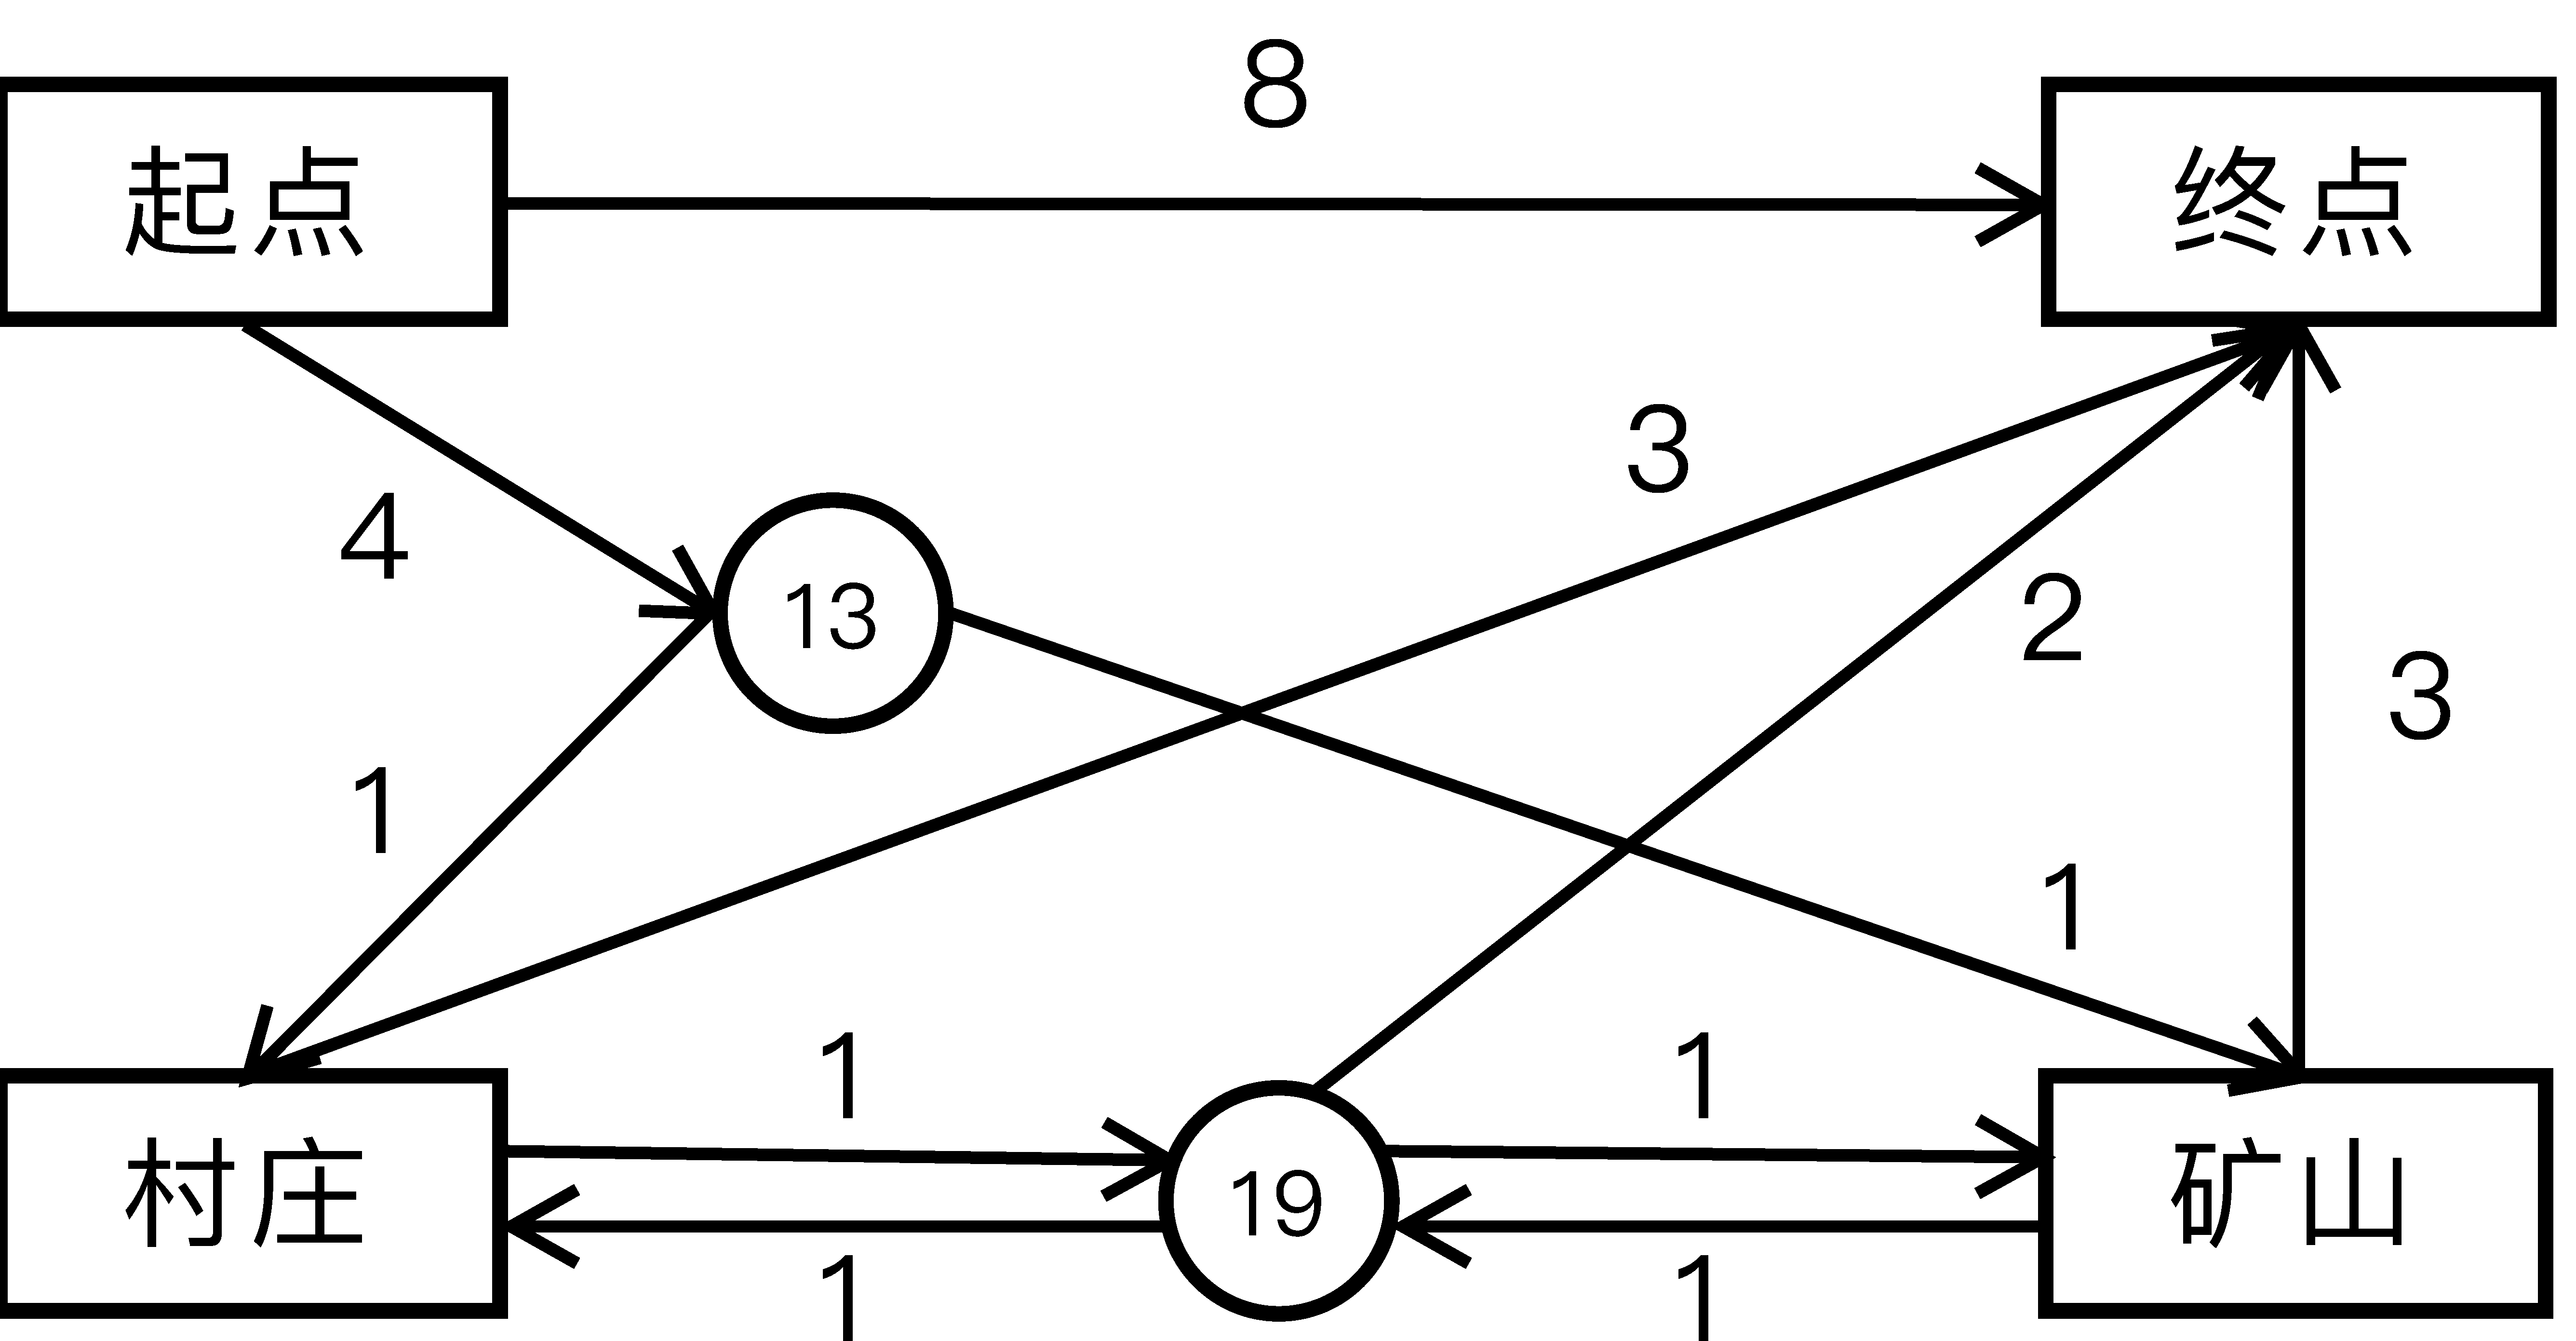
\includegraphics[width=.5\textwidth]{problem4-network}
    \caption{第四关-模型简化}
    \label{fig:problem4-network}
\end{figure}

箭头上的数字代表了两个结点之间的最短需要花费的时间(最短距离),每个结点上用户均可决定等待或前进。

% 最终可以建立出一个更为简单的模型,该模型只考虑关键节点,即用户可能会作出的不同决策的位置。

\subsection{符号说明}

% 本文所使用的变量符号及其含义如表\ref{tab:sign}所示。

\begin{table}[!htbp]
    \caption{本文符号}\label{tab:sign} \centering
    \begin{tabular}{p{1.5cm}p{3cm}|p{1.5cm}p{3cm}|p{1.5cm}p{3cm}}
        \toprule[1.5pt]
        符号 & 含义 & 符号 & 含义 & 符号 & 含义\\
        \midrule[1pt]
        $cost$ & 花费 & $m_{init}$ & 初始资金 & $w_{cost}$ & 水的基准价格 \\
        $cap_{basic}$ & 基础收益 & $c_{total}$ & 总计花费  & $f_{cost}$ & 食物的基准价格 \\
        $w_{sun}$ & 晴天基础耗水 & $w_{hot}$ & 高温基础耗水 & $w_{dust}$ & 沙暴基础耗水 \\
        $f_{sun}$ & 晴朗基础耗食物 & $f_{hot}$ & 高温基础耗食物 & $f_{dust}$ & 沙暴基础耗食物\\ 
        $m_{left}$ & 剩余的钱 & $f_{left}$ & 剩余的粮食 & $w_{left}$ & 剩余的水 \\
        $f_{buy}$ & 购买的粮食 & $w_{buy}$ & 购买的水 & $d_{total}$ & 总的天数 \\ 
        $d_{cur}$ & 当前天数 & $point$ & 玩家位置 & $k$ & 阶段数 \\
        $s_k$ & 第$k$个阶段状态 & $x_k$ & 第$k$个阶段决策 & $D$ & 决策集合 \\ 
        $d_{min}$ & 绕道矿山到终点 & $cap_{total}$ & 全部收益  & $cost_{total}$ & 全部花费   \\
        $c_{sun}$ & 晴朗基础消费 & $c_{hot}$ & 炎热基础消费  & $c_{dust}$ & 沙尘基础消费    \\
        \bottomrule[1.5pt]
    \end{tabular}
\end{table}

同时,我们用$distance(i,j)$表示点区域i到区域j的最短的路径,其中i和j是小于区块总数的正整数。


\subsection{模型假设}

\label{sub:assumption}

为了更好解决问题,我们对模型作出部分预设:

\begin{enumerate}
    \item 沙尘暴较少指沙尘暴不影响正常的行走,部分情况下视做三天或四天之内至多出现一次沙尘暴。
    \item 玩家在已知对方策略的博弈过程中,存在不同的博弈倾向。
\end{enumerate}



\section{全程天气状况已知条件下的最优策略}
\label{sec:simulate}

\subsection{分析}
在本问题中,整个游戏时段内每天天气状况事先全部已知,且游戏的时间有限制,即游戏在有限步内结束。因此,玩家行动策略的总数是有限的,其中必然存在一个最优策略。对于策略总数有限的问题,可以通过穷举法找出其中的最优策略。然而,本问题中游戏策略众多,单纯使用穷举法的计算量过大。使用\textbf{动态规划}方法,将多阶段决策问题中的决策序列(整体策略)转化为若干子策略,可以有效减少计算量。

\subsection{模型建立}
\subsubsection{有向图模型}
在本问题中,只有一名玩家,不存在玩家之间的博弈问题。又因为沙漠中所有区域的天气相同,除了起点、终点、村庄、矿山以外的区域是等效的,玩家只需要重点关注起点、终点、村庄、矿山所在的区域。根据\ref{subsec:shortest}小节所述的方法,本问题中第一关和第二关的地图可以分别简化为如图?和图?所示的有向图。
\subsubsection{动态规划模型}
\begin{enumerate}
\item 阶段变量

考虑到游戏规则中“以天为基本时间单位”,选取“天”为动态规划的分段依据,动态规划的阶段数与游戏中的当前天数相等,即
\begin{equation}
    k=d_{cur}
\end{equation}

\item 状态变量

用$s_k$表示第$k$阶段的状态集合,每个状态由玩家所处的位置、所携带资源(水和食物)的数量决定。
\begin{equation}
    s_k=g(point,w_{left},f_{left})
\end{equation}

$s_k$满足无后效性,即$s_k$一旦确定,从该阶段到游戏结束时的最佳策略(即从$s_k$出发的最佳子策略)不受第$k$阶段以前各阶段状态的影响。一旦各个阶段的状态都确定,整个游戏过程也就完全确定。

\item 行为决策

用$x_k(s_k)$表示第$k$个阶段玩家处于$s_k$状态时的决策,$D_k(s_k)$表示第$k$阶段玩家处于$s_k$状态时允许的决策集合,故$x_k(s_k) \in D_k(s_k)$。根据游戏规则,可枚举出玩家处于不同状态时的决策集合。以第一关中玩家处于矿山(12号点)的状态为例,决策集合可表示如下:

\begin{table}[!htbp]
    \caption{第一关中玩家处于矿山时的决策集合}\label{tab:decisions} \centering
    \begin{tabular}{cccc|cccc}
        \toprule[1.5pt]
        决策编号 & 天气 & 路径 & 是否挖矿 & 决策编号 & 天气 & 路径 & 是否挖矿\\
        \midrule[1pt]
        $A_1$ & 晴朗 & 移动至11号点 & 否 & $E$ & 高温 & 停留 & 是\\
        $B$ & 晴朗 & 停留 & 是 & $F$ & 高温 & 停留 & 否\\
        $C$ & 晴朗 & 停留 & 否 & $G$ & 沙暴 & 停留 & 是\\
        $D_1$ & 高温 & 移动至11号点 & 否 & $H$ & 沙暴 & 停留 & 否 \\
        \bottomrule[1.5pt]
    \end{tabular}
\end{table}

在动态规划中,对于每一阶段、每一状态,可计算出具体的决策集合。

\item 状态转移函数

每个阶段,玩家可能会发生资源和位置的变化,导致状态变化。状态转移函数如公式(\ref{state1})-(\ref{state2})所示。

\begin{equation}
    w_{left}=
    \begin{cases}
        w_{left}-n*w_{sun}& s_k \in \text{\{晴朗\}}\\
        w_{left}-n*w_{hot}& s_k \in \text{\{高温\}}
        \\
        w_{left}-w_{dust}& s_k \in \text{\{沙暴\}}
    \end{cases}
    \label{state1}
\end{equation}
\begin{equation}
    f_{left}=
    \begin{cases}
        f_{left}-n*f_{sun}& s_k \in \text{\{晴朗\}}\\
        f_{left}-n*f_{hot}& s_k \in \text{\{高温\}}
        \\
        f_{left}-f_{dust}& s_k \in \text{\{沙暴\}}
    \end{cases}
\end{equation}

\begin{equation}
    s_{k+1}=g(point_{k+1},w_{left},f_{left})
    \label{state2}
\end{equation}

在公式(\ref{state1})-(\ref{state2})中,
\begin{equation}
    n=
    \begin{cases}
        3 & s_k \in \text{\{挖矿\}}\\
        2 & s_k \in \text{\{移动\}}\\
        1 & s_k \in \text{\{停留\}} \cap \text{\{不挖矿\}}\\
    \end{cases}
\end{equation}


\item 阶段损益函数

游戏的目标是在到达终点的前提下尽可能多保留资金,将资金的变化作为阶段损益函数。
\begin{equation}
    cost(s_k,x_k)=-p*w_{cost}*w_{buy}-p*f_{cost}*f_{buy}+q*cap_{basic}
\end{equation}
其中,
\begin{equation}
    p=
    \begin{cases}
        2 & s_k \in \text{\{补给\}} \& k \neq 0\\
        1 & k=0 \\
        0 & else
    \end{cases}
\end{equation}
\begin{equation}
    q=
    \begin{cases}
        1 & s_k \in \text{\{挖矿\}}\\
        0 & else
    \end{cases}
\end{equation}
\end{enumerate}
基于以上说明,动态规划模型可总结为:
\begin{equation}
    \begin{cases}
        cost_{total}(s_0)=m_{init}-m_{left}(s_0) \\
        cost_{total}(s_{k+1})=cost(s_k,x_k)+cost_{total}(s_k) & k=0,1,2,...,d_{total}-1
    \end{cases}
\end{equation}
其中,$x_k \in D_k(s_k)$,$m_{left}(s_0)$为第0天补给后的剩余资金。

遍历最后一阶段中所有处于终点位置的状态,总计花费最少(剩余资金最多)的策略序列即为该初始状态下的最优策略。模型求解中,将考虑具体关卡的所有初始状态,以得到该关卡的全局最优策略。

\subsection{模型求解}
\subsubsection{算法简述}
由于在起点处(第0天)存在不同的物资补给策略,这些策略会影响初始状态,进而影响游戏过程中的决策序列和最终结果。因此,使用\textbf{多重搜索}算法分别考虑第0天水和食物的补给,对第0天的所有补给策略进行搜索,每种补给策略对应一个初始状态。确定初始状态后,使用动态规划模型计算出每种初始状态所对应的最优策略。最后,从所有初始状态所对应的最优策略中选出最优策略,即为关卡的全局最优策略。

在有村庄的地图中,村庄补给的策略过多大大增加了计算复杂度。因此,采用“先使用后记账”的策略对算法进行优化:允许资源存在缺口,每次经过村庄或到达终点时,若资源存在缺口,则检查缺口是否可在上一次经过村庄时得到满足。若可以满足,则补上缺口,扣除资金,保证了补给的最低限度;若无法满足(超过负重或上次经过村庄时资金不足),则进行\textbf{剪枝},停止此状态的继续递推。此外,考虑到模型的求解方向和状态转移函数的方向均为正向,求解过程中结合了\textbf{记忆化搜索}算法对经典动态规划算法加以改进。

算法使用Python进行实现,源代码见附录。
\subsubsection{第一关}
通过多重搜索后,不同初始补给条件下最优策略的最终资金如图\ref{p1_global}所示。最终资金为0(深蓝色)的区域表示:这些初始补给条件下的资源数量超过负重上限或不足以支持玩家到达终点。
\begin{figure}
    \centering
    \includegraphics[width=12cm]{p1_global.eps}
    \caption{第一关:不同初始补给条件下最优策略的最终资金}
    \label{p1_global}
\end{figure}

经计算,第一关的最优策略为:第0天携带178箱水和333箱食物出发;第8天到达村庄并补给163箱水;第10天到达矿山,第11至19天在矿山停留,其中第11、17天不挖矿,其他日期挖矿;第21天再次到达村庄并补给36箱水和16箱食物;第24天到达终点,水和食物均刚好用尽;最终剩余资金10470元。详细计算结果见附录。
\subsubsection{第二关}
具体求解过程与第一关类似,不再赘述。经计算,第二关的最优策略为:第0天携带130箱水和405箱食物出发;第10天到达位于点16(原始地图中区域39)的村庄并补给10箱水;第11天停留在该村庄并补给179箱水;第12天到达位于点17(原始地图中区域30)的矿山;第13至18天在该矿山挖矿;第19天到达位于点16的村庄并补给196箱水和86箱食物;第21天到达位于点11(原始地图中区域55)的矿山;第22至28天在该矿山挖矿;第30天到达终点,水和食物均刚好用尽;最终剩余资金12730元。详细计算结果见附录。

\begin{figure}
    \centering
    \includegraphics[width=12cm]{p2_global.eps}
    \caption{第二关:不同初始补给条件下最优策略的最终资金}
    \label{p2_global}
\end{figure}

\section{天气未知情况下一般的最佳策略}
\label{sec:simulate}

\subsection{问题分析}

在仅仅知道当天天气的情况下,玩家的最佳策略的主要约束条件是 :在保证游戏不失败的前提下,最大化游戏收益。
为了不保证游戏失败,玩家必须在指定的的时间内到达终点,同时保证仍然有水和食物剩余,这就需要玩家合理安排购买的物品以及在矿
山开矿的时间。

影响决策的最主要的因素是沙尘暴天气和炎热天气的比例,以及是否有村庄。
沙尘暴天气的出现概率小于100\%,否则玩家将无法前进;
炎热天气的概率为0\%-100\%,即可能一路上全部是炎热,也可能全部是晴朗;
村庄可能有,也可能没有;
矿山在该问题中预设是存在的,否则不需要研究如何最大化利益。


\begin{table}[!htbp]
    \caption{影响因素情况}\label{tab:001} \centering
    \begin{tabular}{c|cccc}
        \toprule[1.5pt]
        影响因素 & 沙尘暴天气 & 炎热天气 & 村庄 \\
        \midrule[1pt]
        变量范围 & 0\%-99\% & 0\%-100\% & 有/无 \\
        \bottomrule[1.5pt]
    \end{tabular}
\end{table}


% 以上的因素都会影响最佳决策的设计,比如如果没有村庄,则只需要考虑如何能够最优化在矿山的收益,以及如何
% 安全地到达终点,其决策路径必定是“起点$\to$前往矿山$\to$挖矿/休息$\to$终点”,或者直接“起点$\to$
% 终点”。
我们接下来将对模型进行简化,然后对决策因素的影响进行分析,考虑在部分因素不确定的情况下、部分因素确定的情
况下,一般玩家的最优决策。

\subsection{模型建立}

% 该模型的建立基于两个预设条件:
% (1)玩家能够在起点购买物品后,一次性到达终点。
% (2)玩家从起点到终点所需要花费的最小时间,略小于总的允许时间。
% 我们可以基于这两个假设条件,先对网络模型进行简化,将问题简化为决策路径确定情况下,如何最优化资源利用
% 效率的问题。

\subsubsection{网络模型简化}
\label{subsub:simplify}

根据\ref{subsec:shortest}的推导与附录A的算法,我们可以将网络进行预先简化为只有关键结点的模型。
以第四关为例,玩家需要从起点前往“矿山”或“终点”,为了实现最优策略,避免走路造成更多的消耗,途中必然会
选择最短路径,途中的大部分位置是等价的。
但是在13/19位置,玩家可以决定是先前往矿山还是村庄、是继续挖矿还是前往终点,这也是关键结点。

% 最短路径中会存在交集,比如前往矿山和村庄的最短路径中可以在13位置相交、村庄和矿山到终点的最短路径在19
% 号位置相交,在13/19号位置可能会产生决策行为,即是先前往矿山还是村庄、是继续挖矿还是前往终点。
% 根据\ref{subsec:shortest}小节的证明,我们可以通过最短路径算法,将路径简化为:

\begin{figure}[!h]
    \centering
    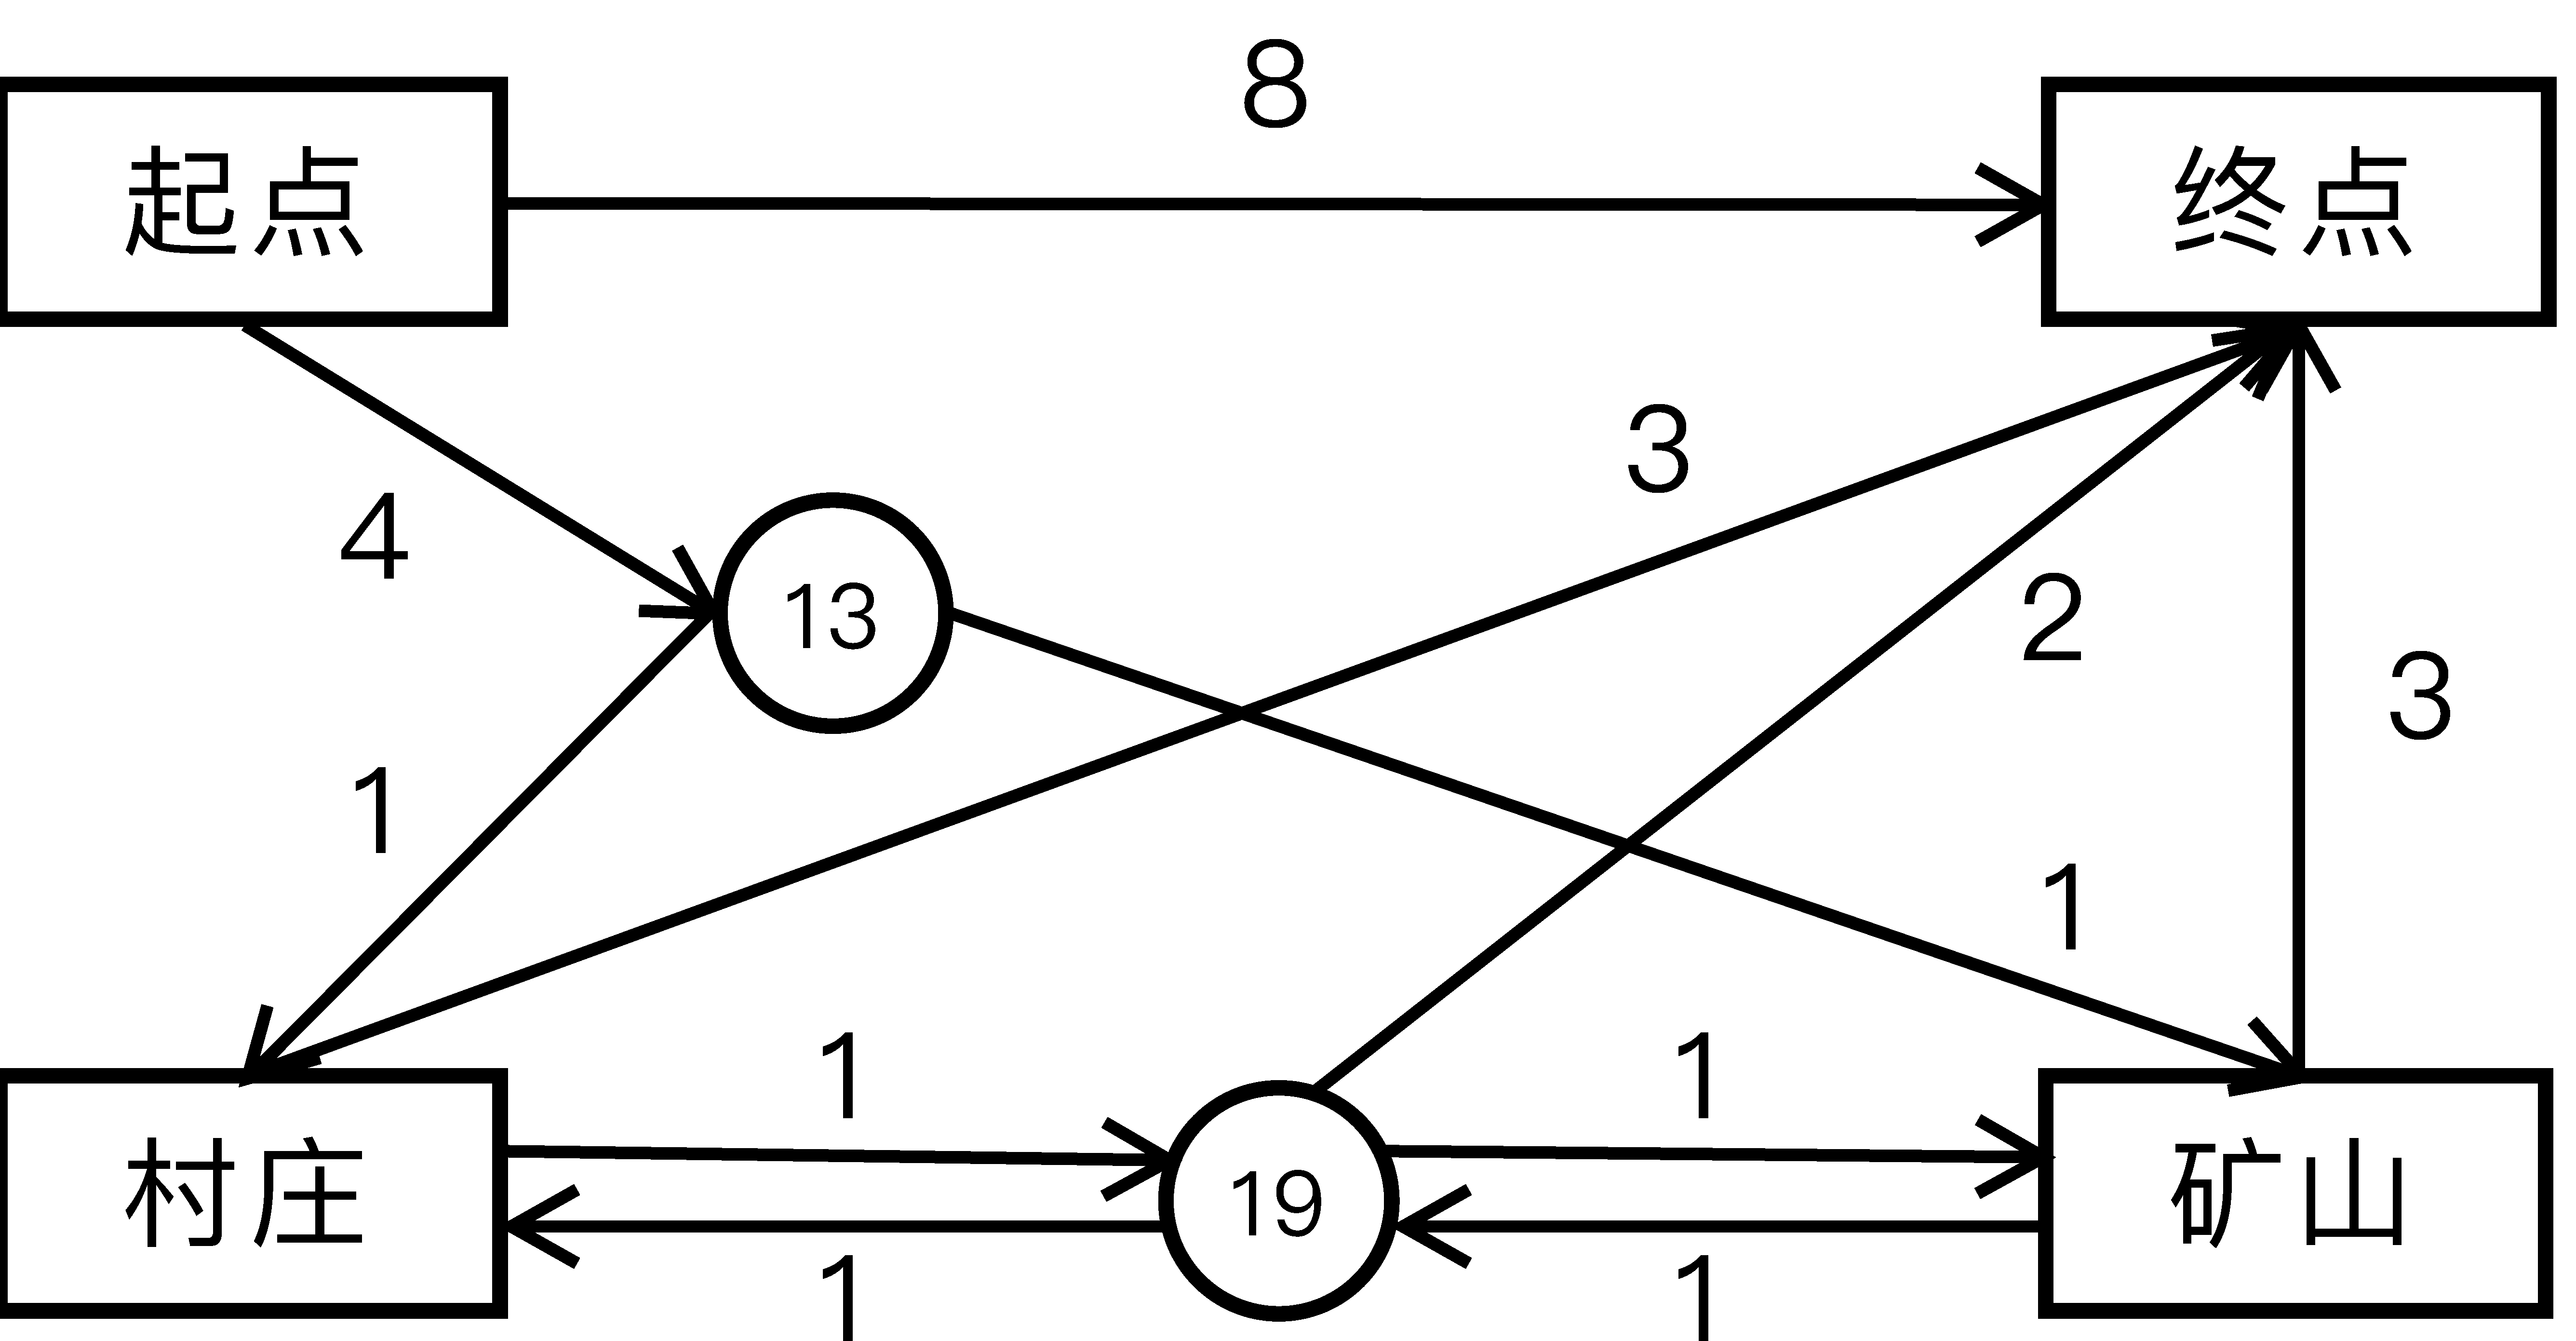
\includegraphics[width=.5\textwidth]{problem4-network}
    \caption{第四关-模型简化}
    \label{fig:example-network}
\end{figure}

\noindent 在这个图中,箭头上的数字代表两个地点之间需要行走的区块,在这些区块中玩家可以选择行走或
停在原地。
同时,玩家到达“矿山”后可以选择停下不工作或“挖矿”。
由于玩家重新回到“起点”无法购买,而前往“终点”游戏结束,所以不存在从“矿山”前往“起点”或“终点”前往其
他位置的直线。


% \uline{在这个模型中,虽然我们没有考虑是否应该选择矿山和终点的中间路径,然后根据遇到的天气决
% 定是否前往矿山或终点,但是后续我们会说明,该简化方式不会影响我们的最优策略分析。}

\subsubsection{决策路径建立}

建立好简化版的网络模型后,我们可以建立玩家的一般决策路径,包括决策的各个阶段和各自的触发条件,然后
再量化比较不同路径的效果,从而得出最优策略。

% 同样以第四关为例,根据\cref{subsub:simplify}介绍的简化模型,我们可以将其转化为下述的决策过程:

\begin{figure}[!h]
    \centering
    
\includegraphics[width=.85\textwidth]{problem4-decision}
    \caption{第四关-决策路径}
    \label{fig:example-decision}
\end{figure}
\uwave{决策路径一般分为两个方向:(1)直接前往终点,包含直接终止阶段(2)绕行前往矿山后再前往终点,
包含初始阶段、挖矿阶段和终止阶段。}

同样以第四关为例,图\ref{fig:example-decision}是图\ref{fig:example-network}简化后的决策模型,
玩家可以选择直接前往终点,终止游戏,也可以选择先前往矿山,然后工作或休息,当满足一定的条件,比如携带的
水或食物不够时,触发终止条件,前往终点。


基于该模型,我们可以进行后续的分析,以描述完整的最优决策过程,即:\textbf{玩家应该如何根据条件,选择
“直接终止”(左)或前往矿山或村庄(右);在初始阶段、挖矿阶段、终止阶段,玩家应该依照天气采取怎样不同的
策略;何种条件会触发结束挖矿阶段,开启终止阶段。}

\subsubsection{基于影响因素策略分析}

% 会影响策略的因素主要有,是否有村庄、是否有沙尘暴天气或当天是否沙尘暴天气,和当天是否高温天气,三个因素
% 会对玩家的决策产生影响。

\textbf{(1)村庄影响}

如果没有村庄,那么玩家需要合理安排到矿山的时间以及初始购买的粮食,同时在保证在预期时间能够到达终点;
如果有村庄,玩家需要合理安排在矿山和村庄之间的时间,保证能够在预定时间内到达村庄的情况下最大化收益。

\begin{stratygy}
    在没有村庄时,玩家的决策路径是由起点直接前往终点,或由起点直接前往矿山后再前往终点;在有村庄时,
    玩家决策路径会增加村庄与矿山之间的往返。
    \label{str:hot}
\end{stratygy}

\textbf{(2)高温的影响}

高温天气是沙漠的常见天气,其水和食物的消耗量是普通情况的2-3倍,而行走或挖矿过程中,消耗量更大。
同时,由于未来的天气情况是未知的,如果高温天气当天不走,未来可能仍然是高温,所以在非矿山的位置,玩家
都应该不管与否高温直接前往目的地。
在矿山位置所做的决策则应该取决于资源成本、天气、村庄及其距离等因素。

% 在挖矿阶段,如果热天挖矿的总花费大于等于挖矿基准收益$3*cost_{hot} \geq cap_{basic}$,应该放弃在热天挖
% 矿;如果总花费小于总收益$3*cost_{hot} < cap_{basic}$,热天可能可以挖矿,具体应该取决于是否有村庄、资源
% 购买费用、村庄距离等因素。

\begin{stratygy}
    在非挖矿阶段,玩家玩家应该不管高温与否直接前往目的地;在挖矿阶段,应该对收益与成本进行量化分析。
    \label{str:hot}
\end{stratygy}

\textbf{(3)沙尘暴的影响}

沙尘暴的影响与高温类似,主要区别在于,沙尘暴的基础消耗量比高温天气更高,同时沙尘暴天气下能够挖矿(也消
耗三倍的食物和水)、沙尘暴天气下无法行走。
沙尘暴天气只能够留在原地或挖矿,所以沙尘暴主要会产生两个影响:需要提前前往终点以保证按时到达终点、需要
根据成本、利润决策是否应该挖矿。

\begin{stratygy}
    如果有沙尘暴天气,若玩家选择挖矿,应该提前前往终点;是否在沙尘暴天气挖矿取决于实际收益是否高于支出。
    \label{str:dust}
\end{stratygy}

\subsubsection{决策路径与阶段分析}

% 上一小节我们讨论了几个因素的定性影响,这一节我们要讨论应对不同的条件,玩家应该如何决策路径,以及不同决策
% 阶段玩家应该如何作出决策。

% (1)玩家应该直接前往终点,还是绕路前往矿山挖矿后,再前往终点。
% (2)若前往矿山,玩家应该在多久挖矿、多久前往村庄购买多少物资。
% (3)若前往矿山,出现什么情况玩家应该考虑前往终点。
上一小节我们讨论了几个因素的定性影响,这一小节我们探讨玩家应该如何决策路径,以及不同阶段应该作出的决策,包括应该挖矿
还是终止、什么天气应该挖矿、是否前往村庄、是否前往终点等,最终可以使得剩余的金钱最大化。

该问题的目标为,在初始资金$m_{init}$给定的情况下,最大化最终的剩余的资金$m_{left}$。我们定义可能出现的沙尘暴天数为$d_{dust}$、
绕道挖矿与村庄的总距离$detour$、挖矿天数为$d_{mine}$、后续的总花费$cost_{total}$、挖矿收益$cap_{total}$、起点到终点距离$dis$,
其他参数沿用先前,优化目标可以描述为:
% 需要满足的约束条件为时间不会超出(14)以及资源足够最极端环境到达终点(15-16),


\begin{alignat}{2}
    \max \quad & m_{left} = m_{init} - cost_{total} + cap_{total}, \\
    \mbox{s.t.}\quad
    &cost_{total} = (w_{buy}+w_{village}*2)*w_{cost} + (f_{buy}+f_{village}*2)*f_{cost},  \\ 
    &cap_{total} = d_{mine}*cap_{basic} ,\\ % 获得的前
    &d_{total} \geq dis + detour + d_{dust} + d_{mine}, \\ % 时间约束
    &w_{buy}+w_{village} \geq w_{hot}*(d_{mine}*3+dis_{cur}*2+detour*2) + w_{dust}*d_{dust}, \\ % 资源约束  
    &f_{buy}+f_{village} \geq f_{hot}*(d_{mine}*3+dis_{cur}*2+detour*2) + f_{dust}*d_{dust} % 资源约束  
\end{alignat}

我们可以看到最终的收益决定于在起点和村庄购买资源的花费(12),以及挖矿的总收益(13),同时时间(14)和资源(15-16)都需要满足游
戏不失败的约束,基于此目标函数,我们可以总结出一下四个策略。

% 当前天数为$d_{cur}$、玩家当前到终点最近距离为$dis_{cur}$
% \begin{alignat}{2}
%     \max \quad & m_{left} = m_{init} - cost_{total} + cap_{total}, \\
%     \mbox{s.t.}\quad
%     &cost_{total} = w_{buy}*w_{cost} + f_{buy}*f_{cost} ,  \\ 
%     &cap_{total} = d_{mine}*cap_{basic} ,\\ % 获得的前
%     &dis_{cur} \le d_{total} - d_{cur} - detour - d_{dust} - d_{mine}, \\ % 时间约束
%     &w_{left} + w_{buy} \geq w_{hot}*(d_{mine}*3+dis_{cur}*2+detour*2) + w_{dust}*d_{dust}, \\ % 资源约束  
%     &f_{left} + f_{buy} \geq f_{hot}*(d_{mine}*3+dis_{cur}*2+detour*2) + f_{dust}*d_{dust} % 资源约束  
% \end{alignat}
% 最终,可以看到最终剩余的资金与花费和收益都有关系,花费取决于xxxx,收益取决于xxxx,所以最终需要满足以下五个策略:

\begin{route}
    如果前往矿山可能可以挖矿获得的收益,不足以弥补绕道的成本和无法挖矿时多消耗的水和粮食的费用,则不应该前往
    矿山。
    \label{route:choose}
\end{route}

\begin{route}
    有村庄的情况下是否应该挖矿取决于水和粮食的购买、前往村庄和矿山的综合成本,如果成本合算,参考剩余天数购
    买水和粮食。
    \label{route:country}
\end{route}

\begin{decisionend}
    如果携带的资源刚好在极端天气能够到达终点,且无法额外购买,则需要即刻前往终点。
    \label{deci:day1}
\end{decisionend}

\begin{decisionend}
    如果出现沙尘天气,需要根据距离与剩余时间,提前1-2天前往终点。
    \label{deci:day2}
\end{decisionend}

其中的路径选择1-2的含义为,只有在绕道挖矿能产生正收益且收益能够弥补绕道的费用,挖矿才是划算的;以及只有在绕道
前往村中购买资源,使得能够多产生的收益,能够弥补绕道前往村庄的费用和购买资源的费用,前往村庄才是划算的。
终止条件1-2则表示需要保证游戏能按时成功的结束。
在具体讨论中应该沿用该策略,通过比较潜在收益、剩余资源等因素,考虑最终应该采取的路径与策略。

% 我们简化中间路径,比如\ref{fig:problem3-decision-mid}展示了包含完整路径的第三关决策路径,的确
% 有一定可能会带来最佳结果的缺失。

% \begin{figure}[!h]
%     \centering
%     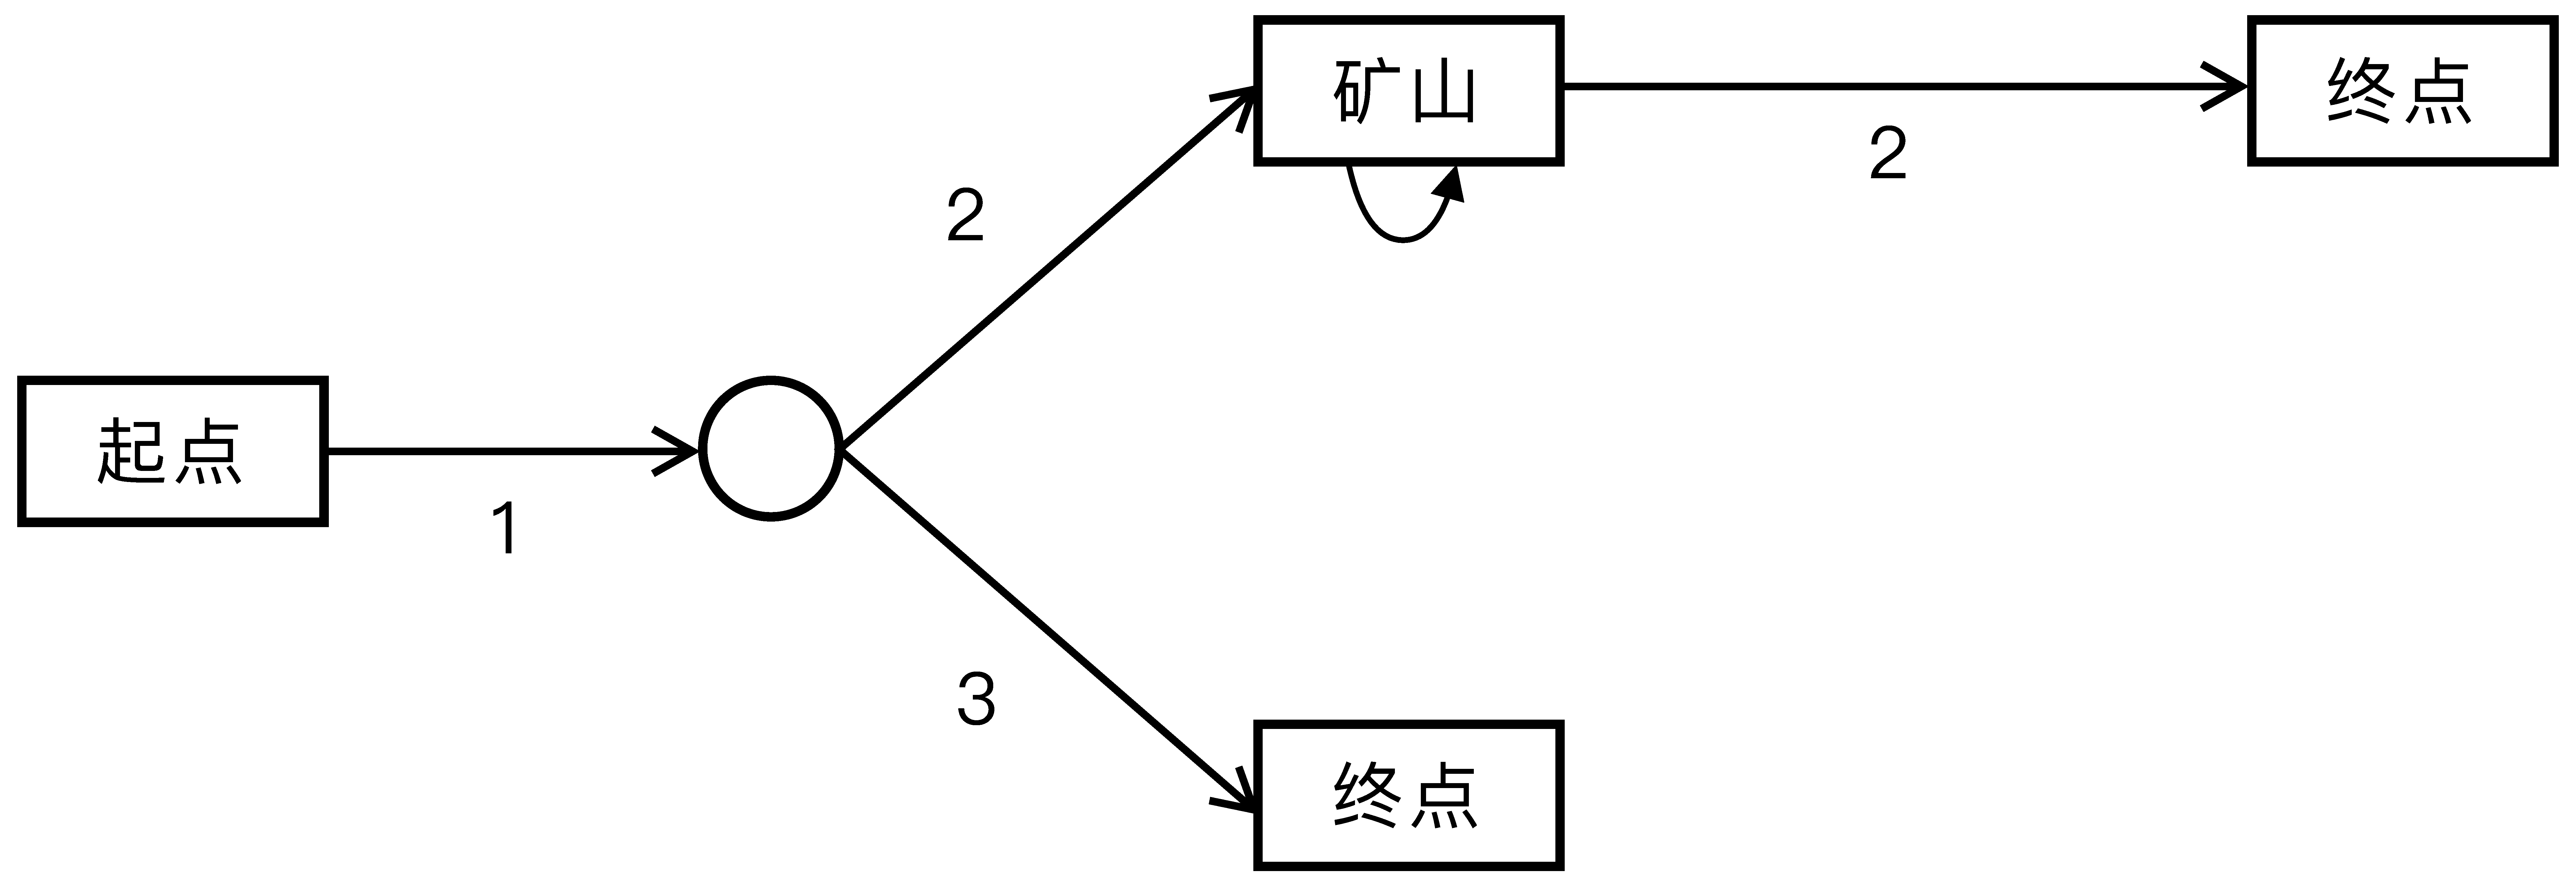
\includegraphics[width=.8\textwidth]{problem3-new-decision}
%     \caption{第三关-考虑中间结点的决策路径}
%     \label{fig:problem3-decision-mid}
% \end{figure}

% 但是根据上面分析可以看到如果收入、花费和绕道的路径满足特定条件,且仅知道当前的天气,未来的天气是未知
% 的,不需要考虑中间路径。
% 因为前往哪里只决定于收益和成本的关系,不决定于某一天当天的的天气,当天的天气只会影响在挖矿阶段用户
% 的决策。




\subsection{模型求解}

\subsubsection{第三关}

第三关中玩家到矿山和终点的最短路径中有一个公共位置4,简化后的模型如图\ref{fig:problem3-network}所示,
具体决策路径如图\ref{fig:problem3-decision}所示。
主要考虑的问题是,到达4位置后是否应该前往挖矿、什么样的天气应该挖矿、以及挖矿阶段的终止条件等。

\begin{figure}[!h]
    \centering
    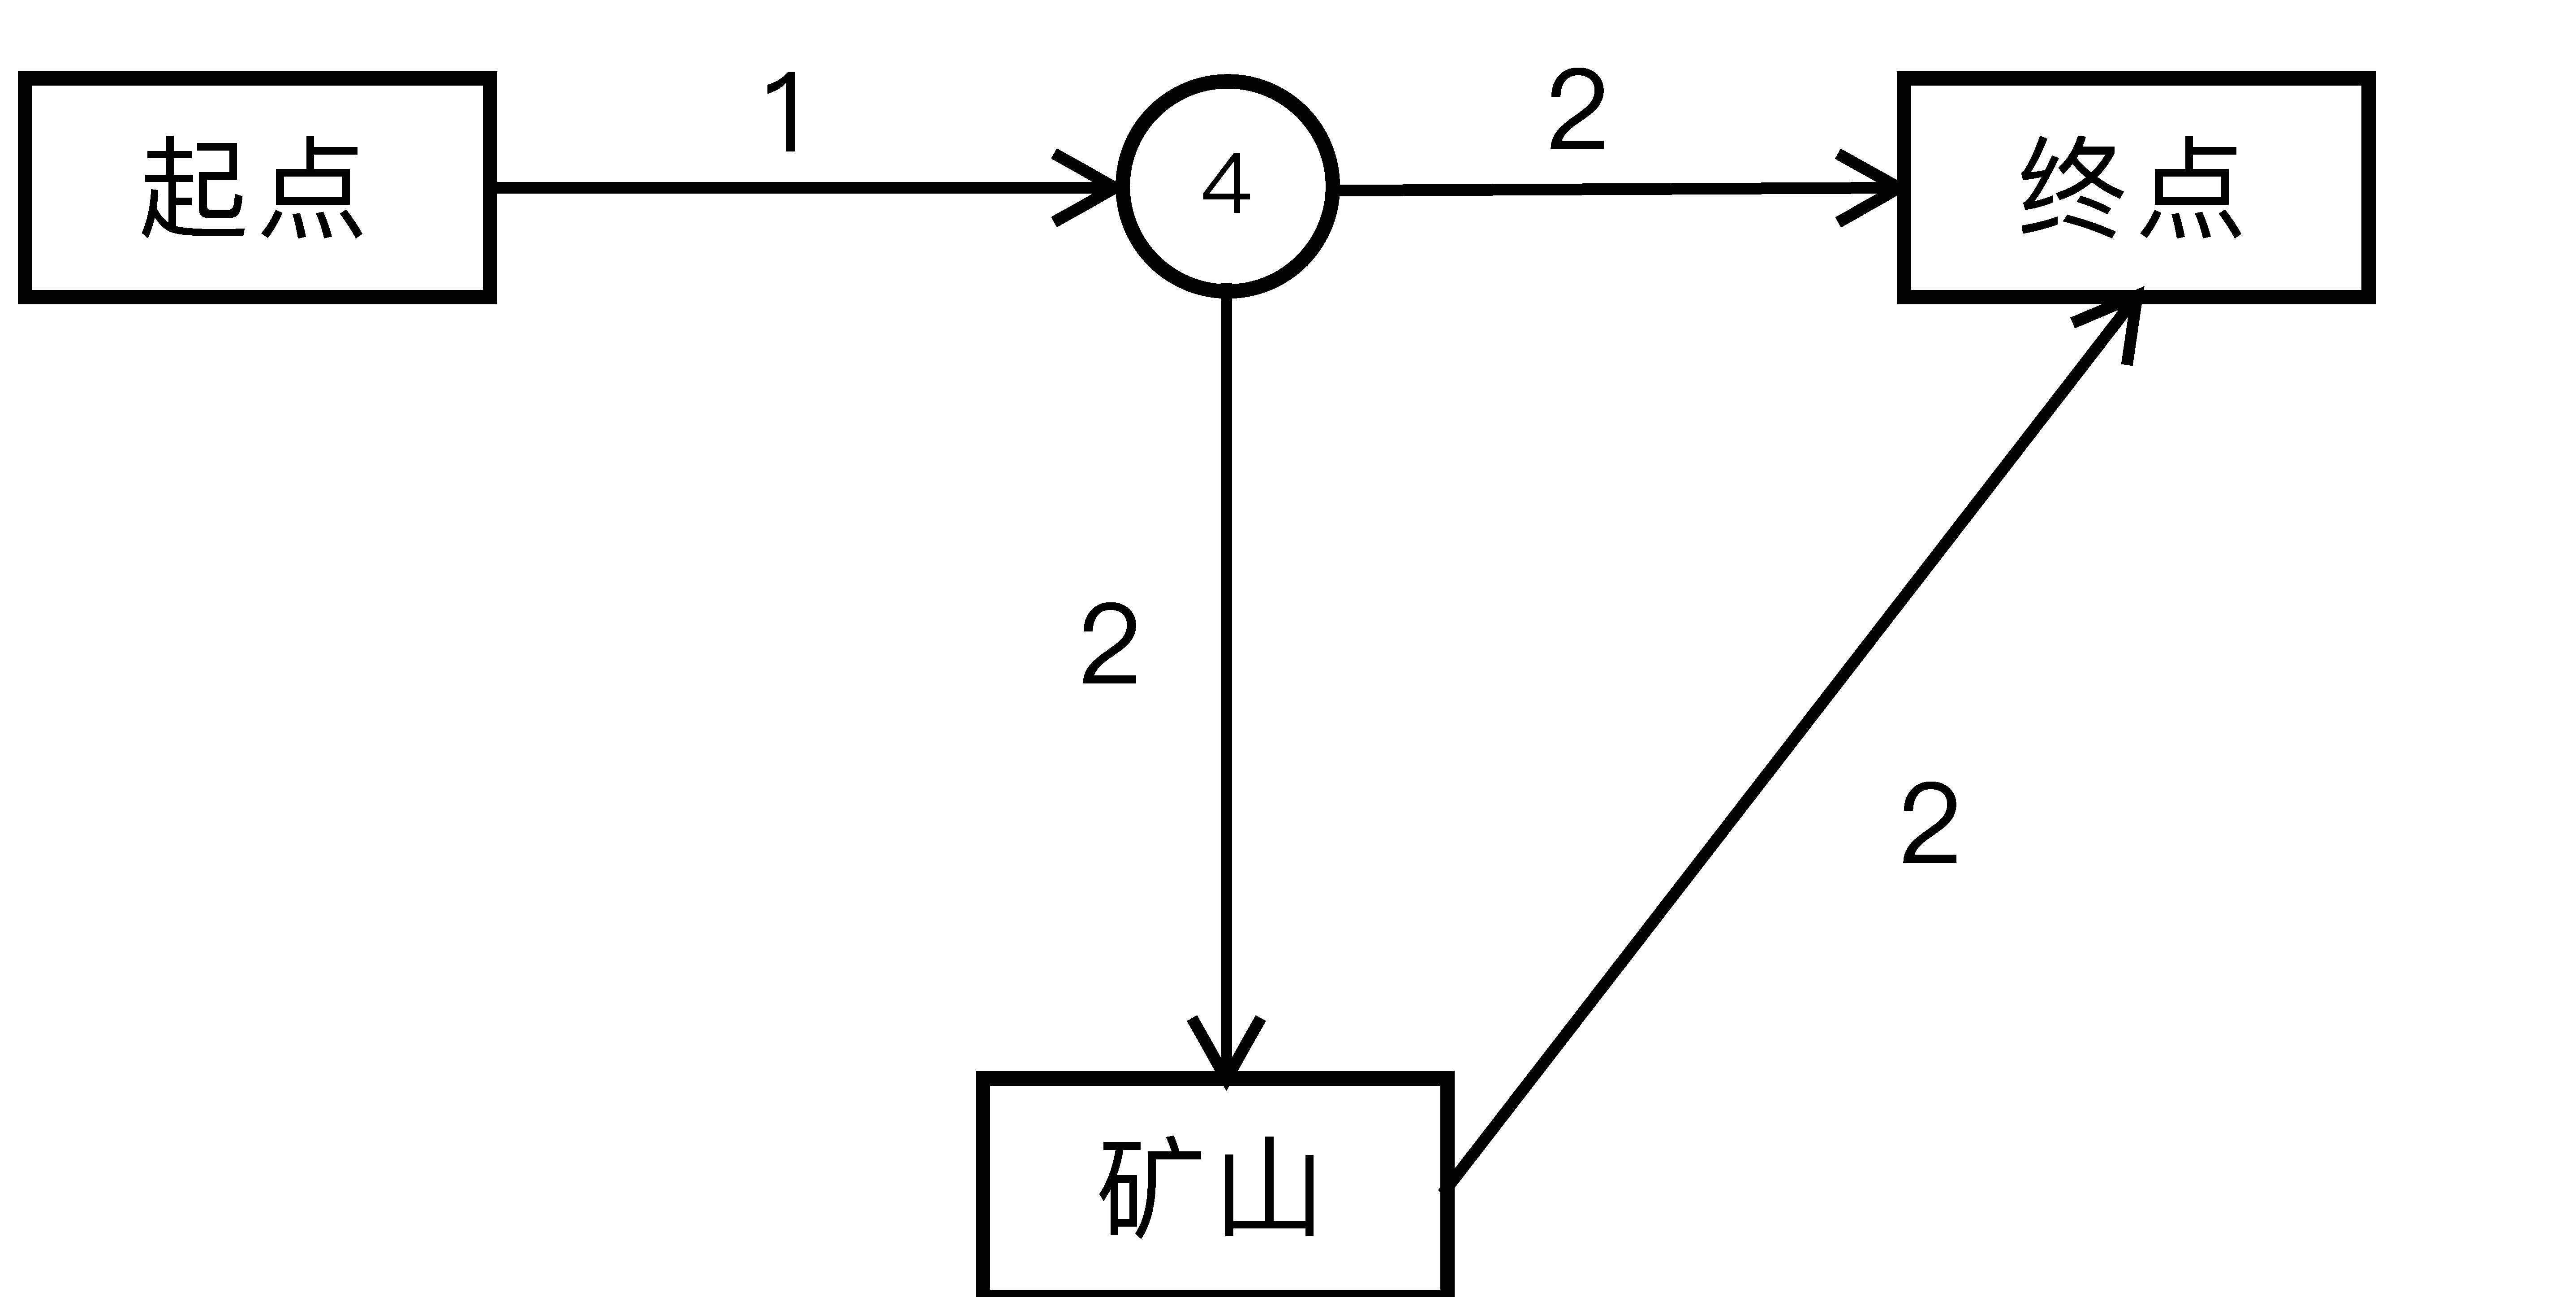
\includegraphics[width=.5\textwidth]{problem3-network}
    \caption{第三关-模型简化}
    \label{fig:problem3-network}
\end{figure}

\begin{figure}[!h]
    \centering
    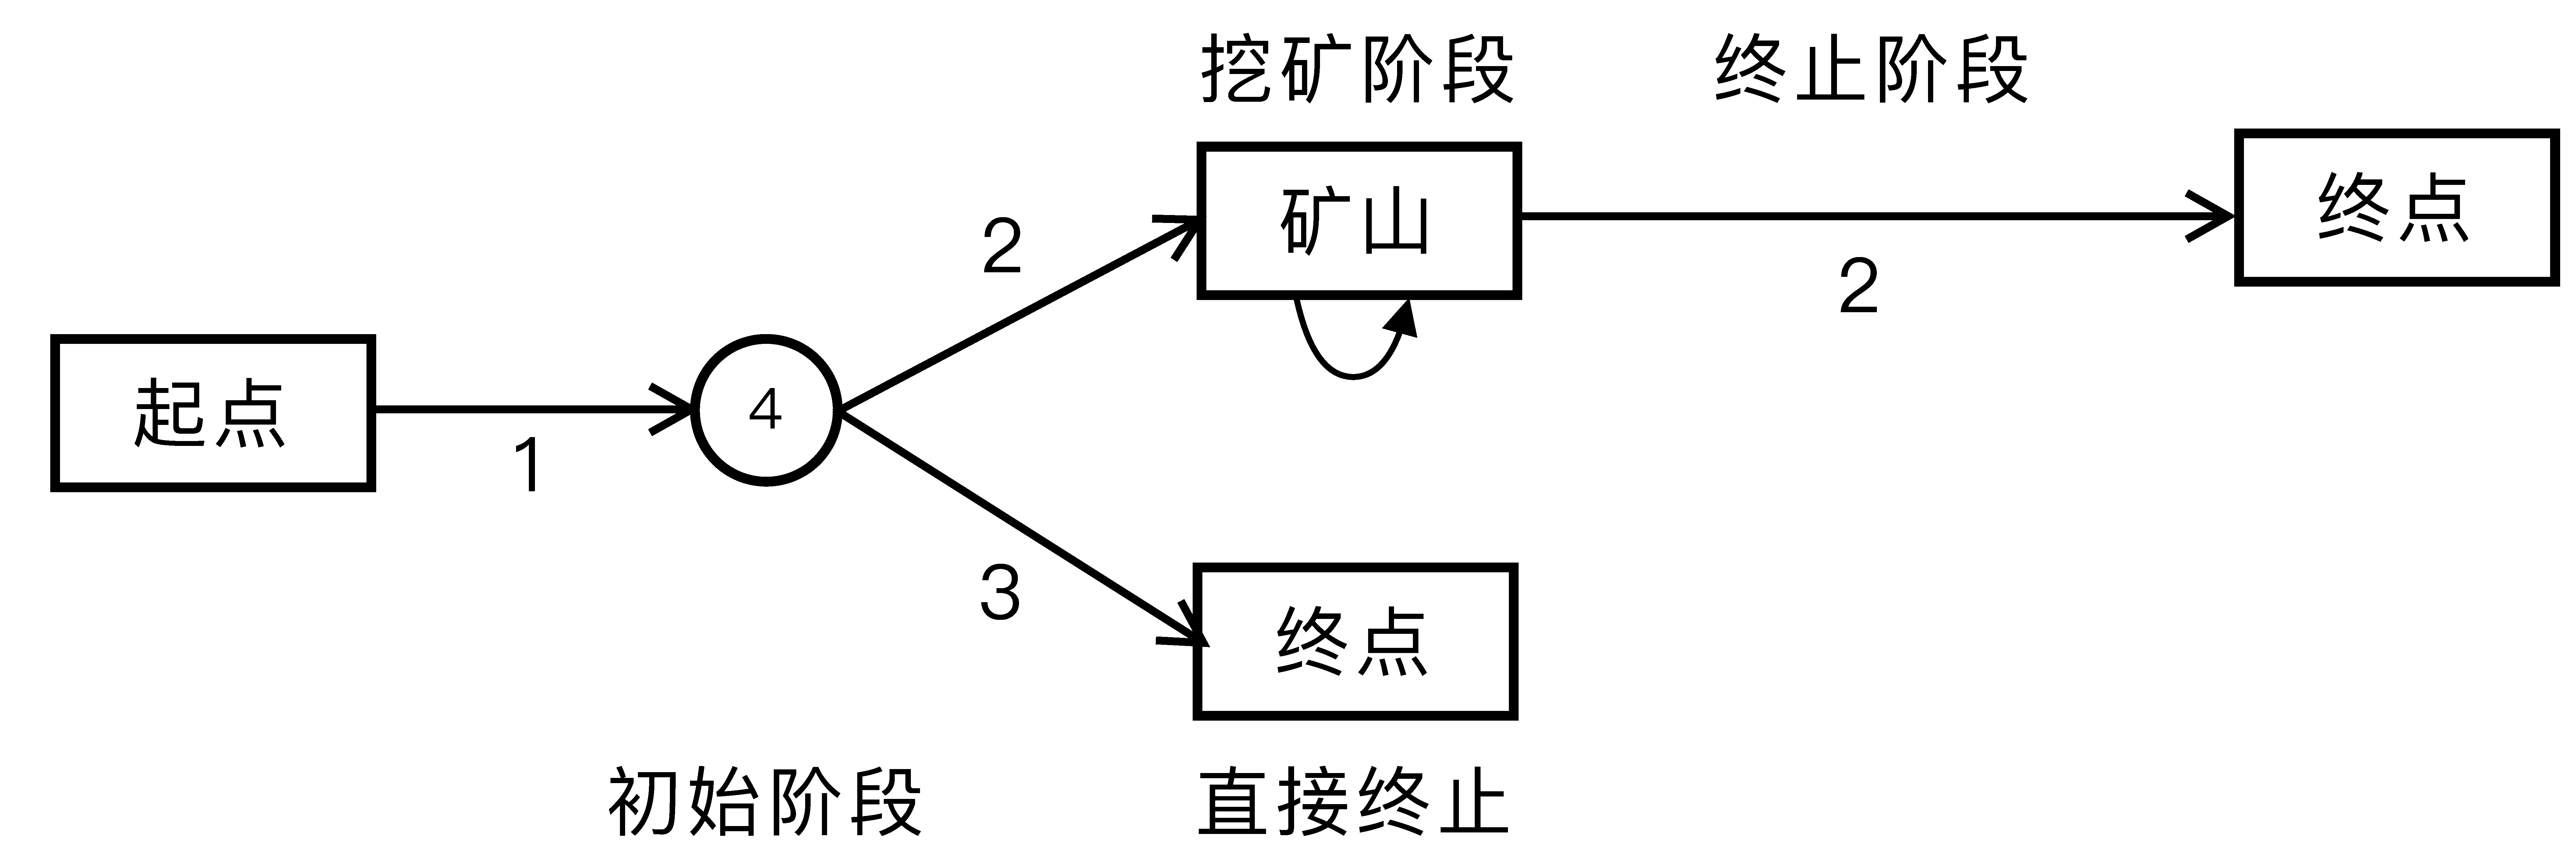
\includegraphics[width=.8\textwidth]{problem3-decision}
    \caption{第三关-决策路径}
    \label{fig:problem3-decision}
\end{figure}

\textbf{(1)成本分析}

该关的基础参数如有,基础收益:$cap_{basic} = 200$元;挖矿绕道距离:$detour = 1$个区块;晴天基础花
费:$c_s=125$元;高温基础花费:$c_{hot}=315$元;总天数$d_{total}=10$天;绕道矿山到终点的最短时
间$d_{min}=5$天。

绕道最高成本$detour*c_{hot}*2=630$元;晴天挖矿收入:$cap_{basic}-3*cost_s=-175$元;热天挖矿
收入:$cap_{basic}-3*cost_h=-745$元;可挖矿天数:$d_{total}-d_{min}=5$天。

\textbf{(2)决策路径分析}

根据上一小节信息,可以比较明显的看到,以挣钱为目的的挖矿是亏损,所以应该准备直接前往终点的资源。
水:$w_{hot}*2*d_{min}=216kg$,粮食:$f_{hot}*2*d_{min}=144kg$。

玩家到达4后需要第一次做决策,如果第1天是晴天,相当于节约了水$(w_{hot}-w_{sun})*2=36kg$,节约了食物
$(f_{hot}-f_{sun})*2=20kg$。

如果到达4后仍然为晴天,则相当于共节约水73kg和食物40kg,由于$detour=1$,所以可以选择绕行到矿山,即前往
3位置,因为即使该天为高温,也能够满足热天走路水54kg和粮食36kg的需求。

玩家到达3后如果再次出现晴天,走到矿山相对于相当于再次节约了水36kg和粮食20kg;到达9矿山后,如果再次出现
晴天,由于上一天节约的水和粮食足够在晴天挖矿的全部消耗,所以应就地挖矿,挣得基础收益200元。

\begin{figure}[!h]
    \centering
    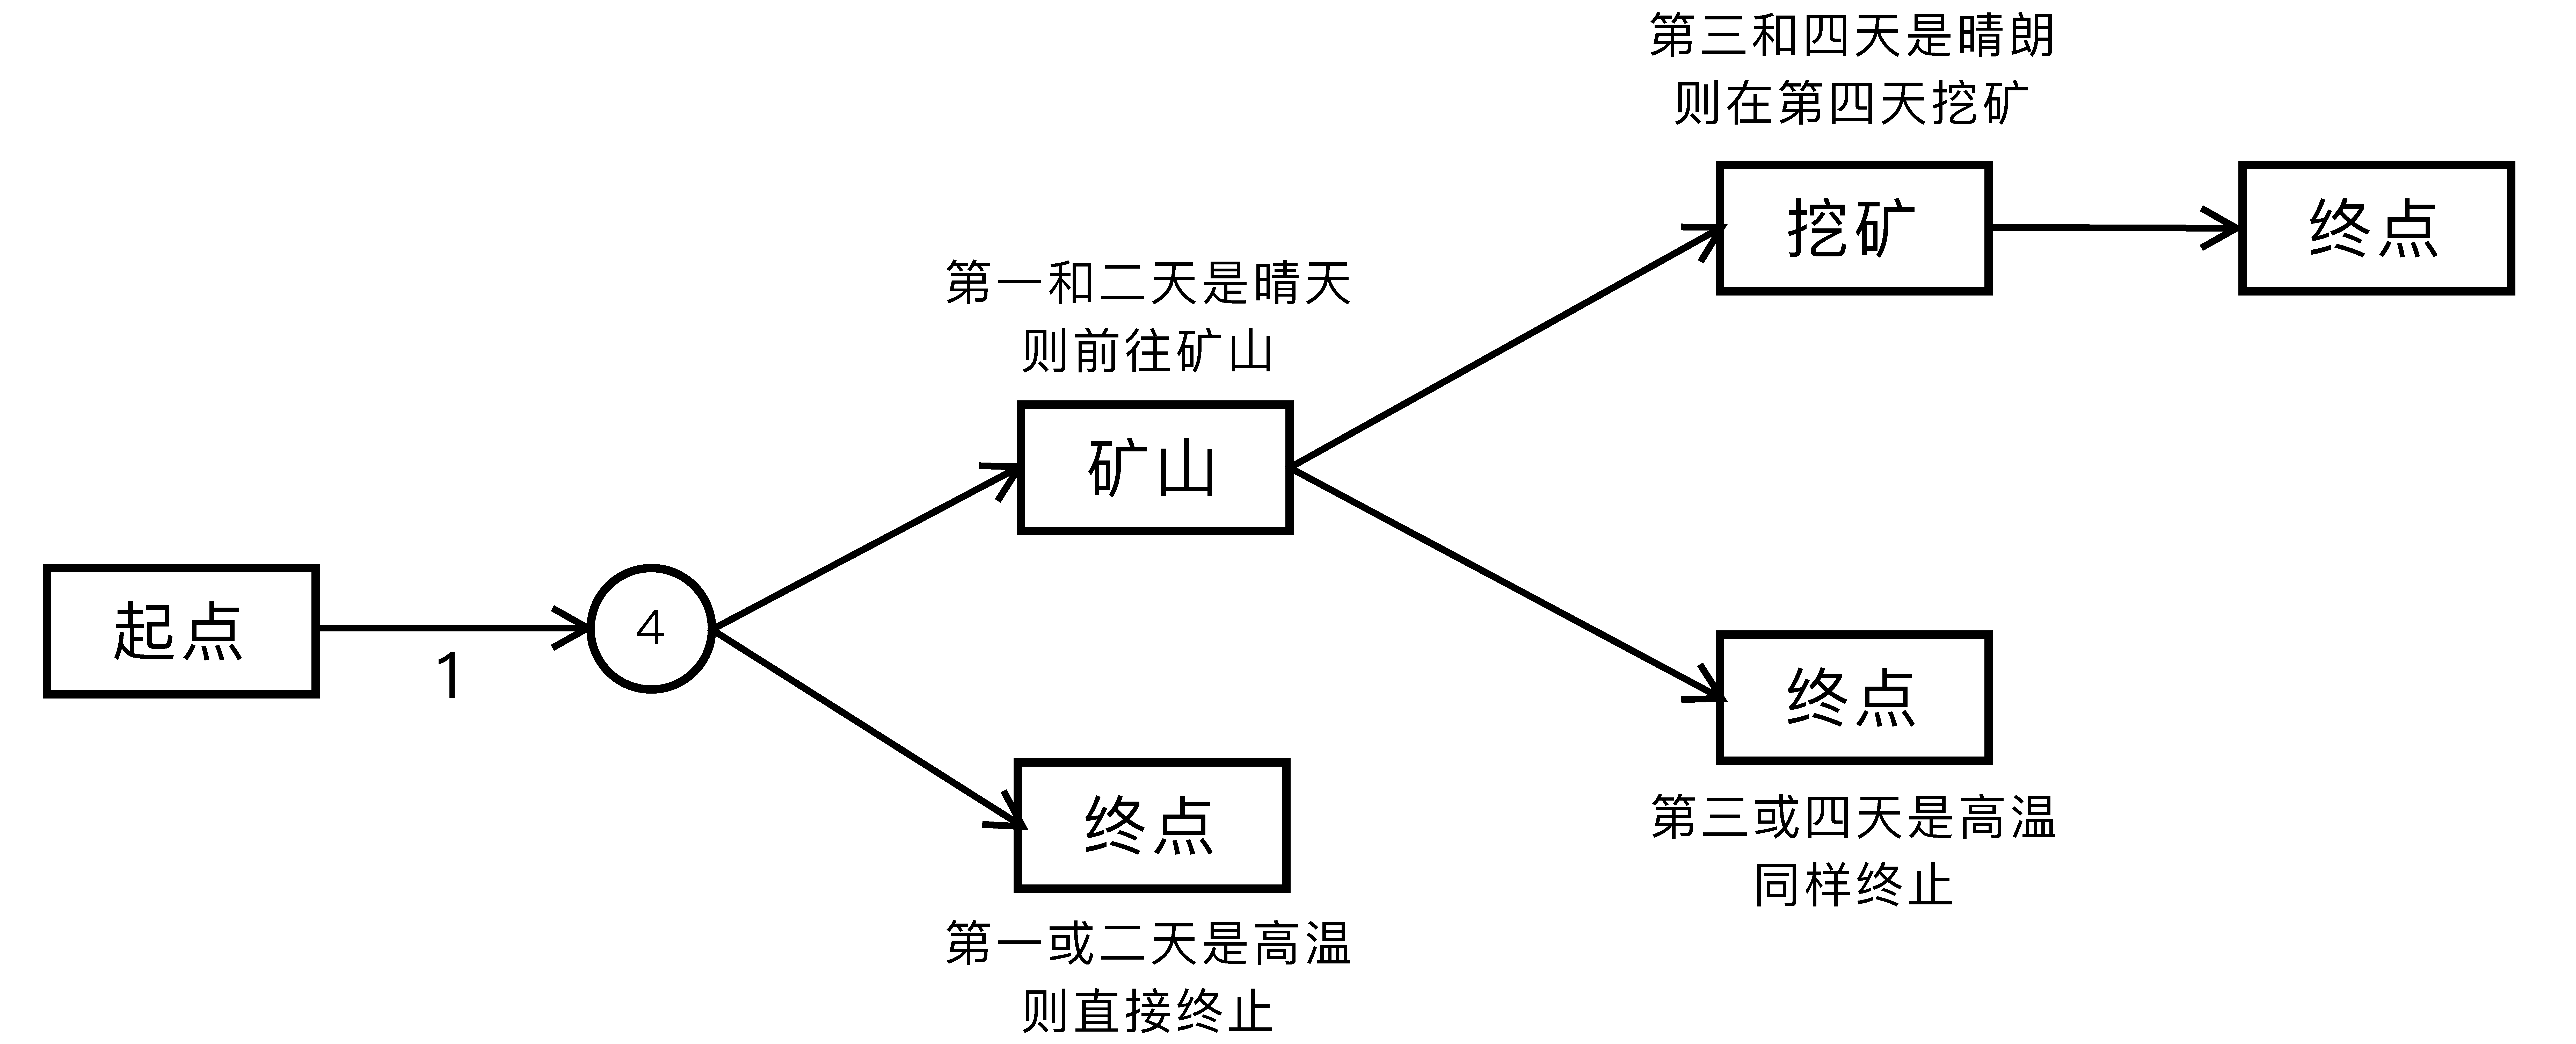
\includegraphics[width=.95\textwidth]{problem3-result}
    \caption{第三关-决策路径选择}
    \label{fig:problem3-result}
\end{figure}

\textbf{(3)策略总结}

上一小节计算出的决策路径呈现的结果即为,准备4天高温行走的粮食和水,如果第1-4天全部为晴天,则在第四天挖矿,获得200元收益。
% 初始的购买总花费为$c_{total} = w_{buy}*w_{cost} + f_{buy}*f_{cost} = 2520$元,购买后剩余资金为
% $m_{left} = m_{init} - c_{total} = 7480$元。

\begin{table}[!htbp]
    \caption{第三关最佳策略}\label{tab:strategy} \centering
    \begin{tabular}{p{2cm}p{13cm}}
        \midrule[1pt]
        初始购买 & $4*w_{hot}=216kg$水和$4*f_{hot}=144kg$的食物,花费2520元 \\
        基本策略 & 第1天前往4号位置,如果第二天是高温,则沿4-6-13到终点;如果第二天不是高温,则按照4-3-9-11-13到终点,其中如果第3/4天全部是晴朗,则在第四天早矿山挖矿 \\
        剩余资金 & 如果没有挖矿,则剩余$m_{init}-216kg*w_{cost}-144kg*f_{cost}=7480$元;如果能够挖矿,则剩余7480+200=7680元 \\
        \bottomrule[1pt]
    \end{tabular}
\end{table}





\subsubsection{第四关}

该问题我们已经进行过分析,其决策路径如下图,需要对其在矿山的挖矿成本进行量化后,判断其在几个核心的决策
结点,应该作出什么决策,同时计算何时触发模型终止策略。

\begin{figure}[!h]
    \centering
    
\includegraphics[width=.9\textwidth]{problem4-decision}
    \caption{第四关-决策过程}
    \label{fig:problem4-decision}
\end{figure}

\textbf{(1)成本分析}

该关的基础参数如有,基础收益:$cap_{basic} = 1000$元;仅挖矿绕道距离:$detour = 0$个区块;
晴朗天气基础消费$c_{sun}=125$元,炎热天气基础消费$c_{hot}=315$元,沙尘暴天气基础消费$c_{hot}=350$元

收入方面,由于在村庄购买的物品价格翻倍,挖矿获得的收入应该分为起点购买的资源用完前,和资源用完后。
在资源用完前,与第三关结果一致,晴天挖矿挣635元,高温挖矿挣55元,同时沙尘暴挖矿损失50元;
资源用完后,晴天收益为$cap_{basic}-c_{sun}*2*3=370$元,高温挖矿收益$cap_{basic}-c_{hot}*2*3=-890$元,
沙尘暴挖矿收益为$cap_{basic}-c_{dust}*2*3=-1100$元。

\textbf{(2)决策路径基础分析}

% 该问题的路径决策主要有,是否应该挖矿、应该先去村庄还是矿山、什么天气可以在矿山挖矿、是否应该去及多久应该去
% 村庄、在村庄应该购买多少资源、多久应该前往终点。

使用起点购买的资源在矿山挖矿时,天晴和高温的净收益分别为635元和55元,虽然沙尘暴天气损失50元,但是题目条件是该天
气比较少,所以在矿山挖矿我们可以视为能够获取收益。
按照天气最恶劣的情况计算,1200kg的负重也足够起点到终点,并剩余可以用来挖矿的资源。
同时$detour=0$,即起点到终点的最短路径是可以经过矿山而无需绕道的,所以玩家应该在起点购买足够的资源,在路过矿山
时直接挖矿以获取收益。

但是在资源耗尽后,高温天气亏损近晴天收益的两倍,同时从矿山前往村庄的过程需要消耗大量资源,玩家也只知道当天的天气,
不知道未来是否是高温,所以完全使用村庄的资源挖矿是不合算的。

% 从起点到矿山一共经过5个区块,最恶劣的天气可以视做消耗5天炎热与1天沙尘暴,共计消耗500kg的资源;
% 从矿山前往终点我们同样预设1次沙尘暴,外加3天高温,共计消耗320kg的资源,初始携带1200kg的食物和水,假设按照1:1
% 携带,也能够剩余足够的资源挖矿。

\uline{综上,玩家一般情况下应该选择最短的路径直接前往矿山挖矿,且不应该存粹使用村庄资源挖矿。}

\textbf{(3)购买策略与决策路径}

在起点处资源的购买应该满足1200kg,考虑到沙尘暴和高温消耗箱数水:食物=1:1,按照该比例购买,恰好水购买720kg,食物
购买480kg。
也可以按照晴朗天气的消耗比例购买,但是由于天气未知,二者差异不大。

在该情况下,如果全部是晴朗天气,水和食物的比例失衡,这时可能可以先前往村庄,再前往矿山,此时的$detour=2$;或在资
源用完后选择前往村庄购买食物,再返回矿山,此时的$detour=4$。
如果到达13号位置时,前4天全部是晴朗,会导致水多出8箱,即使第五天仍然为晴朗,也不应该前往村庄,因为多余的水不足以支
付$detour=2$所花费的可能费用。

如果在矿山挖矿结束前,所有的天气全部为晴天,按照计算共计会行走5天,挖矿11天,按照箱数1:1购买的资源会多出约15个晴
朗天气的耗水,也是5个高温天气耗水。
但是$detour=4$,如果炎热天气,需要多出8个炎热天气的消耗才划算。

所以不管怎么样,都不应该前往村庄购买,最终的具体的决策路径与最佳策略为:

\begin{table}[!htbp]
    \caption{第四关最佳策略}\label{tab:strategy} \centering
    \begin{tabular}{p{2cm}p{13cm}}
        \midrule[1pt]
        初始购买 & 720kg水和480kg的食物,或按照晴朗天气消耗比例 \\
        基本策略 & 直接前往矿山,除了沙尘暴其他天气保持前进,到达矿山后不管天气如何都选择挖矿 \\
        结束条件 & 如果挖矿过程中剩余的水将小于192kg或粮食小于128kg,选择沿最短路径前往终点 \\
        \bottomrule[1pt]
    \end{tabular}
\end{table}

\begin{figure}[!h]
    \centering
    
\includegraphics[width=.7\textwidth]{problem4-result}
    \caption{第四关-决策路径选择}
    \label{fig:problem4-decision}
\end{figure}



\section{多玩家博弈条件下的策略}
\label{sec:simulate}


\subsection{问题分析}

该问题


\subsection{模型建立}

\subsubsection{网络模型}

首先

\subsection{模型求解}

\subsubsection{第五关}


\subsubsection{第六关}






\section{模型评价}
\label{sec:simulate}

\subsection{第一问}

该模型将路径转化为有向图模型后,在一定约束条件和外部环境确定的情况下,建立了完整的动态规划模型,包括
用户决策、状态转移函数、损益函数等,并建立了Python版本的求解算法。
基于该模型,可以直接求解出第一二关的全局最优解。

\subsection{第二问}

该模型分析并建立了简单的网络模型,并分析了在未来情况不确定时的用户最佳决策路径,建立了收益、成本和玩
家行为之间的关系,以及用户的基本行为策略。
基于该模型,给予确定的问题环境,即可直接分析出玩家的最佳行为策略,以及初始的购买需求。

\subsection{第三问}

该模型基于静态博弈与动态博弈的思路,在多玩家参与且决策结果会互相影响的情况下,基于前两问的部分结论,
建立了玩家的行为策略的基本模型。
在环境确定或不确定的情况下,作出能够使得收益最高的决策,达到整体的均衡状态。

%参考文献
\begin{thebibliography}{9}%宽度9
    \bibitem[1]{book:OR}
    沈荣芳.
    \newblock 运筹学\allowbreak[M].
    \newblock 机械工业出版社, 北京, 2015.
    \bibitem[2]{linear}
    Luenberger D G, Ye Y.
    \newblock Linear and nonlinear programming\allowbreak[M].
    \newblock Reading, MA: Addison-wesley, 1984.
    \bibitem[3]{algorithm}
    Cormen T H, Leiserson C E, Rivest R L, et al.
    \newblock Introduction to algorithms\allowbreak[M].
    \newblock MIT press, 2009.
    \bibitem[4]{game}
    Osborne M J, Rubinstein A.  
    \newblock A course in game theory.\allowbreak[M].
    \newblock MIT press, 1994.
\end{thebibliography}






















\newpage

\newpage
%附录
\begin{appendices}

\section{最短路径源码}

这里是附录


\newpage


    \section{动态规划源码}
    
    这里是附录
    
\end{appendices}
    
\end{document} 